\documentclass{article}
\usepackage{amsmath}
\usepackage[utf8]{inputenc}
\usepackage{float}
\usepackage{epsfig,graphicx}
\usepackage{xcolor,import}
\usepackage[german]{babel}

\begin{document}


\thispagestyle{empty}
			\begin{center}
			\Large{Fakultät für Physik}\\
			\end{center}
\begin{verbatim}


\end{verbatim}
							%Eintrag des Wintersemesters
			\begin{center}
			\textbf{\LARGE WINTERSEMESTER 2014/15}
			\end{center}
\begin{verbatim}


\end{verbatim}
			\begin{center}
			\textbf{\LARGE{Physikalisches Praktikum 1}}
			\end{center}
\begin{verbatim}




\end{verbatim}

			\begin{center}
			\textbf{\LARGE{PROTOKOLL}}
			\end{center}
			
\begin{verbatim}





\end{verbatim}

			\begin{flushleft}
			\textbf{\Large{Experiment (Nr., Titel):}}\\
							%Experiment Nr. und Titel statt den Punkten eintragen
			\LARGE{1. Messen - Messfehler}	
			\end{flushleft}

\begin{verbatim}

\end{verbatim}	
							%Eintragen des Abgabedatums, oder des Erstelldatums des Protokolls
			\begin{flushleft}
			\textbf{\Large{Datum:}} \Large{17.10.2014}
			\end{flushleft}
			
\begin{verbatim}
\end{verbatim}
							%Namen der Protokollschreiber
		\begin{flushleft}
			\textbf{\Large{Namen:}} \Large{Veronika Bachleitner, Erik Grafendorfer}
			\end{flushleft}

\begin{verbatim}


\end{verbatim}
							%Kurstag und Gruppennummer, zb. Fr/5
			\begin{flushleft}
			\textbf{\Large{Kurstag/Gruppe:}} \Large{Fr/1}
			\end{flushleft}

\begin{verbatim}






\end{verbatim}
							%Name des Betreuers, das Praktikum betreute.
			\begin{flushleft}
			\LARGE{\textbf{Betreuer:}}	\Large{SETMAN}	
			\end{flushleft}
%		\begin{figure}[!h]
%\def\svgwidth{70mm}
%\import{section1/}{nonne.eps_tex}
%\end{figure}
$\pm$
%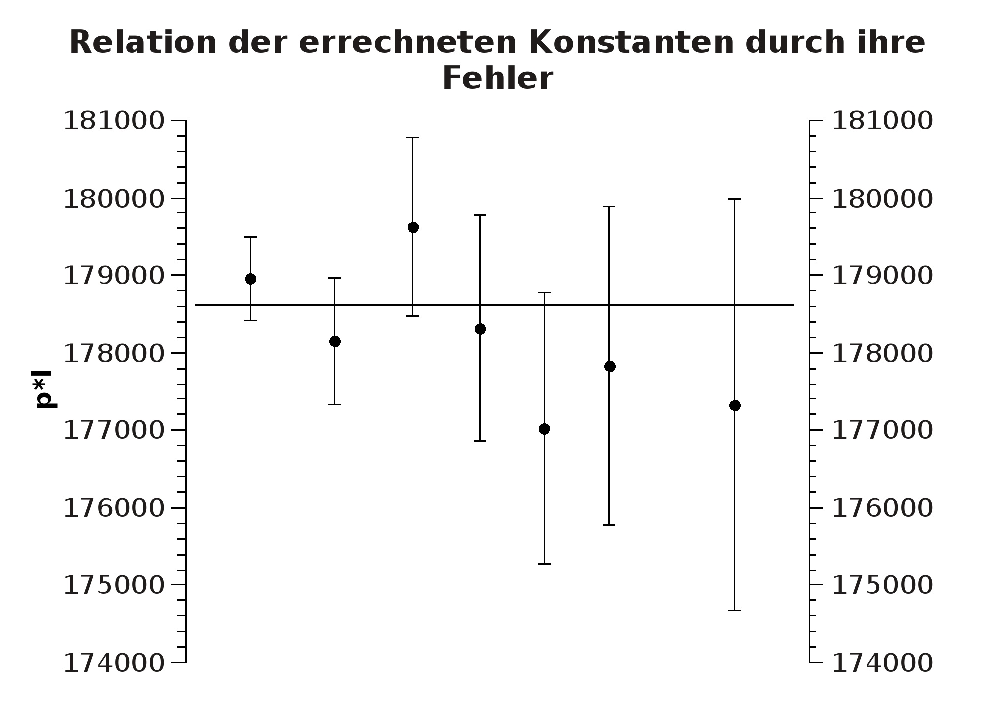
\includegraphics[scale=1,angle=-90]{Graph1.eps}[!h]
\section{Pendel}	
\subsection{Aufgabenstellung}
Es soll die Erdbeschleunigung aus Messungen der Periodendauer eines einfachen Fadenpendels bestimmt werden. Dazu werden 2 Messreihen durchgeführt: Einmal 10 Einzelmessungen als Messreihe; einmal eine Messung von 10 aufeinander folgenden Schwingungen.
\subsection{Grundlagen zum Experiment}
Das Fadenpendel stellt die experimentelle Näherung an ein mathematisches Pendel dar. Bei einem mathematischen Pendel ist die gesamte Masse im Schwerpunkt, die Aufhängung ist starr und reibungsfrei, sowie masselos.
\subsubsection*{Berechnung der Erdbeschleunigung}
Aus der Schwingungsdauer des Pendels können wir uns die lokale Erdbeschleunigung g näherungsweise berechnen. Wir verwenden für kleine Auslenkungswinkel $\alpha$ die Näherung Sin[$\alpha$] $\approx$ $\alpha$. 
Für die Schwingungsdauer T, die Frequenz f und die Pendellänge l gilt:

\begin{align}
T=\frac{1}{f}=2 \pi\sqrt{\frac{l}{g}} \\
g=4\pi^2\frac{l}{T^2}
\end{align}
\subsection{Material und Methoden / Versuchsaufbau}

\subsection{Durchführung des Experiments}

\subsection{Ergebnisse}
Wir berechnen die Unsicherheit der Erdbeschleunigung $\Delta g$ in Abhängigkeit von den gemessenen Größen laut dem Gaußschen Fehlerfortpflanzungsgesetz. Wir berechnen diese 2 Mal, nachdem wir unterschiedliche Näherungswerte und Unsicherheiten für die Schwingungsdauer erhalten wenn wir sie 10 Mal einzeln oder 10 Mal in Folge messen.
\begin{align}
\Delta g=\sqrt{(\frac{\delta g}{\delta l})^2\Delta l^2 + (\frac{\delta g}{\delta T})^2\Delta T^2}
\end{align} \\
Für die 10 Einzelmessungen ist
\begin{equation}
T_{Einzel,genaehert} = (1.93 \pm 0.02)s
\end{equation}
Damit:
\begin{equation}
\Delta g_{Einzel,genaehert} = 0.067 \frac{m}{s^2}
\end{equation}


\begin{equation}
T_{Serie,genaehert} = (1.94 \pm 0.01)s
\end{equation}
Damit:
\begin{equation}
\Delta g_{Serie,genaehert} = 0.0376 \frac{m}{s^2}
\end{equation}
\begin{table}
\begin{center}
Messungen einzelner Schwingungen\\

\begin{tabular}{|c|c|}
\hline \\
Durchgang & Schwingungsdauer[($\pm$0.02s)]\\
\hline 1&1.96\\
\hline 2&1.93\\
\hline 3&1.87\\
\hline 4&1.95\\
\hline 5&1.82\\
\hline 6&1.93\\
\hline 7&1.92\\
\hline 8&1.99\\
\hline 9&1.9\\
\hline 10&1.97\\
\hline

\end{tabular} \\
Messung von 10 konsekutiven Schwingungen:\\
19.36 $\pm$0.01s
\end{center}
\end{table}

Wir verwenden die genauesten Paare von Pendellänge und Schwingungsdauer von allen drei Gruppen, plus einem Paar, das uns die Praktikumsleiterin zur Verfügung stellte, um eine lineare Regression über die Pendellängen durch die Quadrate der Schwingungsdauern zu fitten. Wir verwendeten QtiPlot 0.9.8.9 für die Berechnung und die Darstellung. \\
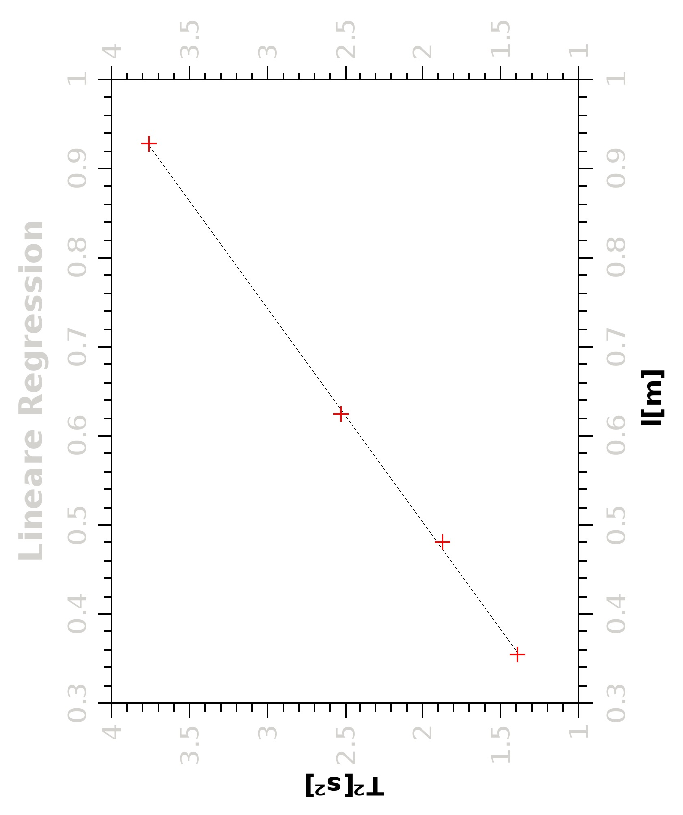
\includegraphics[scale=0.8,angle=-90]{LinearReg.eps}
\subsection{Diskussion}
\section{Mechanische Messungen}
\subsection{Aufgabenstellung}
Es soll der Durchmesser eines Kupferdrahtes mit verschiedenen Methoden gemessen werden. Verwendet werden eine Schublehre, eine Mikrometerschraube und ein Mikroskop mit Okularmaßstab.\\
Ferner sollen 3 Winkel eines Metall-Dreiecks mit einer Winkellehre gemessen werden.

\subsection{Grundlagen zum Experiment}
\subsubsection*{Schublehre}
Mit der Schublehre können Längen mit einer Genauigkeit von 0,05mm gemessen werden. Es gibt eine Hauptskala in Millimeter sowie einen Nonius auf einem beweglichen Schieber. Auf der verwendeten Schublehre sind 20 Teile der Noniusskala auf 39mm der Hauptskala aufgeteilt. Das bedeutet, dass 1mm durch 20 geteilt wird und wir somit die besagte Genauigkeit von 0,05mm erhalten.\\
Um die Ableseregel zu erläutern übernehmen wir eine Abbildung aus dem Anleitungstext, die wir als sehr gut verständlich empfunden haben:\\
(Abbildung!!)

\subsubsection*{Mikrometerschraube}
Mit der Mikrometerschraube können Längen mit einer Genauigkeit von 0,01mm gemessen werden.

\subsubsection*{Mikroskop}

\subsubsection*{Winkellehre}
Um mit der Winkellehre zu messen legt man das zu messende Objekt zwischen die beiden Mess-Schenkel und passt die Schenkel an die Größe an. Das Ergebnis ist wie bei der Schublehre an einer Hauptskala mit Nonius abzulesen.

\subsection{Material und Methoden / Versuchsaufbau}

\subsection{Durchführung des Experiments}

\subsection{Ergebnisse}

\subsection{Diskussion}

\section{Elektrische Messungen}
\subsection{Aufgabenstellung}
Im Gleichstrom messen Ströme und Spannungen in verschiedenen Schaltungen, mal spannungsrichtig, mal stromrichtig, um mit Augenmerk auf die Fehlergrenzen unserer Messgeräte zu sehen, ob wir unsere Messungen wegen der Innenwiderstände der Messgeräte überhaupt korrigieren müssen oder nicht.\\
Weiters messen wir in Parallel- und Serienschaltungen Widerstände und vergleichen sie mit den berechneten Werten.\\
\\
Im Wechselstrom bauen wir einen Spannungsteiler und berechnen Spannungen und Ströme auch in einer modifizierten Schaltung mit einem Kondensator.

\subsection{Grundlagen zum Experiment}
Spannung U: [U]=V (Volt)\\
Stromstärke I: [I]=A (Ampère)\\
Widerstand R: [R]=$\Omega$ (Ohm)\\

Das Ohm'sche Gesetz: U=RI

\subsection{Material und Methoden / Versuchsaufbau}
\includegraphics[scale=0.8,angle=-180]{1stromrichtig.eps}

\subsection{Durchführung des Experiments}

\subsection{Ergebnisse}

\subsection{Diskussion}

\end{document}
